%%%%%%%%%%%%%%%%%%%%%%%%%%%%%%%%%%%%%%%%%%%%%%%%%%%%%%%%%%%%%%%%%%%%%%%%%%%%%%%%
%2345678901234567890123456789012345678901234567890123456789012345678901234567890
%        1         2         3         4         5         6         7         8

\documentclass[letterpaper, 10 pt, conference]{ieeeconf}  % Comment this line out
                                                          % if you need a4paper
%\documentclass[a4paper, 10pt, conference]{ieeeconf}      % Use this line for a4
                                                          % paper

\IEEEoverridecommandlockouts                              % This command is only
                                                          % needed if you want to
                                                          % use the \thanks command
\overrideIEEEmargins
% See the \addtolength command later in the file to balance the column lengths
% on the last page of the document

\usepackage[utf8]{inputenc} 


 
% The following packages can be found on http:\\www.ctan.org
%\usepackage{graphics} % for pdf, bitmapped graphics files
%\usepackage{epsfig} % for postscript graphics files
%\usepackage{mathptmx} % assumes new font selection scheme installed
%\usepackage{times} % assumes new font selection scheme installed
%\usepackage{amsmath} % assumes amsmath package installed
%\usepackage{amssymb}  % assumes amsmath package installed

\title{\LARGE \bf
VisBig : Visualize Big Data in Real Time
}

%\author{ \parbox{3 in}{\centering Huibert Kwakernaak*
%         \thanks{*Use the $\backslash$thanks command to put information here}\\
%         Faculty of Electrical Engineering, Mathematics and Computer Science\\
%         University of Twente\\
%         7500 AE Enschede, The Netherlands\\
%         {\tt\small h.kwakernaak@autsubmit.com}}
%         \hspace*{ 0.5 in}
%         \parbox{3 in}{ \centering Pradeep Misra**
%         \thanks{**The footnote marks may be inserted manually}\\
%        Department of Electrical Engineering \\
%         Wright State University\\
%         Dayton, OH 45435, USA\\
%         {\tt\small pmisra@cs.wright.edu}}
%}

\author{Gonçalo Fialho \\ 
        Instituto Superior Técnico \\
        Universidade de Lisboa \\ 
        Av. Rovisco Pais, 1049-001 Lisboa, Portugal \\
        Email: goncalo.f.pires@tecnico.ulisboa.pt }
    %    \and  
    %    Gonçalo Fialho \\ 
    %    Instituto Superior Técnico \\
    %    Universidade de Lisboa \\ 
    %    Av. Rovisco Pais, 1049-001 Lisboa, Portugal \\
    %    Email: goncalo.f.pires@tecnico.ulisboa.pt 
    %    }

        % <-this % stops a space
%\thanks{*This work was not supported by any organization}% <-this % stops a space
%\thanks{$^{1}$H. Kwakernaak is with Faculty of Electrical Engineering, Mathematics and Computer Science,
%        Instituto Superior Técnico, Universidade de Lisboa, Portugal
%        {\tt\small h.kwakernaak at papercept.net}}%
%\thanks{$^{2}$P. Misra is with the Department of Electrical Engineering, Wright State University,
%        Dayton, OH 45435, USA
%        {\tt\small p.misra at ieee.org}}%
%}
\usepackage{float}

\makeatletter
\let\NAT@parse\undefined
\makeatother

\usepackage[pdftex]{hyperref}

\usepackage{graphicx}

\begin{document}



\maketitle
\thispagestyle{plain}
\pagestyle{plain}


%%%%%%%%%%%%%%%%%%%%%%%%%%%%%%%%%%%%%%%%%%%%%%%%%%%%%%%%%%%%%%%%%%%%%%%%%%%%%%%%
\begin{abstract}

Nowadays information devices can be found anywhere, whether in a personal computer, smartwatch or even in our appliances. These devices create relevant information to the identification of patterns or anomalies of the systems. Given the significant growth of those devices, some representation methods are no longer able to respond efficiently to users needs. Although there are solutions to visualize this type of information it's important to look for new ways to present them in a real-time environment so users can act quickly to the abrupt change of the regular flow of data so they can attempt to solve the problems of the systems. This thesis provides a solution for presenting large amounts of real-time data where users are able to identify anomalies and trends in information as well as maintain context when changes in data flow exist.

We propose \textit{\textbf{VisMillion}}, a visualization interface for large amounts of data in real-time. This web solution is based on \textit{Canvas} technology. Using different modules the system represents data in many ways. The more recent the data, the more detailed it is, so each module uses different techniques to aggregate and process information. 

This report does a state-of-the-art analysis for viewing large amounts of data in real time. Then it presents the architecture of the solution and its justifications for the options taken. Finally, carries out a detailed evaluation of the obtained results and a final analysis and reflection where some of the future work is also mentioned which could improve the system.

Keywords -  Large ammount of data, BigData, Real-Time, Streaming, Visualization, Flow, Trend, Outliers, Patterns

\end{abstract}


%%%%%%%%%%%%%%%%%%%%%%%%%%%%%%%%%%%%%%%%%%%%%%%%%%%%%%%%%%%%%%%%%%%%%%%%%%%%%%%%
\section{INTRODUCTION}


With exponential increase of devices capable of generating information (from the simplest smartphones to supercomputers), it was necessary to find ways to make the visualization simple and effective, so the user won't be misled by elements that are not part of the data. Many systems create a lot of data that must be analyzed, companies like \textit{Amazon} or \textit{Facebook} need to keep track of all the activities performed by the users so they can interpret trends and patterns to create marketing strategies for their business. Robots and Complex Networks generate logs that are important to analyze in case of failures. This is some examples that lead to the emergence of big chunks of information and it is therefore increasingly common to observe the growth of the storage capacity of the devices.

This agglomerated information that creates large chunks of data is typically called as \textbf{Big Data}. However, the term does not have a specific definition and there is no exact value to a dataset can be considered as 'Big Data' \cite{WardB13a}. This data is so large that the tools that process this information cannot do it in a considerable time interval and its necessary to use more efficient methods. One of the most common uses for this kind of data is to visualize it through representations that show patterns and particular details about them. Its representation can be done from a greater degree of detail of each point to aggregations that describe a lot of points with just an element. Yet, the large amounts of data make the discovery of relevant items more difficult causing a more complex and time-consuming analysis. Furthermore its hard to represent all the information just in once because the resolution of the displays could not be enough to represent all the points and Humans have difficulties to understand small parts of data when the datasets are huge, losing the context of their search. To overcome this, data is represented with different levels of detail aggregating information at some point. 

The rise of distributed systems raises this problem to a new scale where it is necessary to monitor real-time changes in case of need for rapid intervention in problems that can occur. The more the servers are the more data will exist and each one has different workload making the amount of data generated by second different and that could cause abrupt changes in the visualization of these systems.

There are challenges that visualization of large amounts of data in real time can arise. First, the processing and rendering phases of this data can be slow. Second, unlike a static environment where the data is always on the same spot, real-time data is constantly coming and there is no way to keep the representation state unmodified and explorable like in a fixed dataset. Third, there is no time to wait for new data to process statistics, this process should always be done the fast as possible so the user could retrieve and get the information to act if necessary. Additionally is important to understand the data domain that is visualized so it can be possible to prevent failures and the systems could adapt to data changes so the users cannot be harmed. 

With this in mind, we have created VisMillion,an interface that represents large amounts of data in real time. Our main goal is to \textbf{provide new information visualization techniques capable of representing large amounts of data in real time that allows the user to perceive the global context of the information as new packages are received}.

The user should be capable to get a global overview of the system and detect interesting patterns using sub visualizations that allows exploring more details about it. To make this happen the information will be aggregated over time so recent data is always more detailed than the old one, using statistical methods the data is represented in many ways. The user should also be capable to identify \textit{outliers} using different methods that are described in the next sections.

The system composed of 3 different modules positioned side by side, each one represents data with a different level of aggregation. Then data flows through each one from right to left. This is built to be suitable with the debit differences and keep updated to all changes that can occur without misleading the user. 

The application was tested using usability user tests with 21 users, using the same approach to all. The results show that the application suits its purpose and the users are capable of analyzing changes, patterns, and anomalies.

The rest of the paper is organized as follows. Section \ref{section:stateofart} we discuss the related work about real time visualization of large amounts of data. In section \ref{section:streammer} is described the global system architecture and server implementation. In section \ref{section:background} we give a overview about the methods and requirements about information visualization. In section \ref{section:frontend} we present the interface VisMillion. In \ref{section:evaluation} the evaluation of the system is described. Finally, in section \ref{section:conclusions} the conclusions of the work are presented as the future work.




\section{State of the art}
\label{section:stateofart}
Applying real-time to data visualization creates new types of challenges \cite{7994551}. First, we need to understand the data domain, this process is called \textit{Orientation} and we should analyze the data behavior and its components. Second, the systems should react efficiently to data changes that are unexpected, this phase is called \textit{Re-Orientation}.

Information Visualization has three characteristics that should be thought of: \textit{Technique}, \textit{Interactivity}, \textit{Data}. The first one is about \cite{981847} the representation of the data (2D, 3D, pixels, etc.). The interactivity refers to how the user should interact with the data to understand the whole system. Data is about its dimensionality and characteristics that influence how data should be presented.

Khan et al. \cite{1878880183} propose a \textit{framework} that interacts with real-time data capable of dealing with intense data flows. This interface is capable to detect anomalies and highlight them. This approach performs dimensional reduction to the data and then using a recommendation system it chooses the suitable representations for the data. The information uses smooth transitions, so the user can maintain the context about the global data view.

Systems like \cite{traub2017i2, 7338157} use dimensional reduction to deal with large datasets, therefore the interfaces doesn't have lots of data to render. These processes are commonly performed at the server side due to connection issues like latency and protocols. Furthermore, there are some complexities associated with performing dimensional reduction and usually they take some time to process, there are some algorithms to perform this quickly on real-time systems.

Some monitoring systems like LiveRac \cite{McLachlan} and X-SimViz \cite{7338157} create solutions that enable users to visualize and analyze clusters of nodes that need to be supervised in case of something bad happen and Human intervention is required. These applications use multiple views, each one uses different levels of detail or present different types of data. Using techniques like \textit{Brushing \& Linking} and \textit{Stretch and Squish Navigation} each part of the interface can communicate with the others and make the context of the data received being preserved.

\textit{Event Visualizer} \cite{Fischer} is a system capable of processing, analyzing and presenting dynamic events in real-time. It uses a module that pre-processes events and makes a search for missing data. Then the interface categorizes each event and each category corresponds to a bar called \textit{relaxed timeline}. There are multiple \textit{relatex timelines} and each one is bound with a different color, its width corresponds to a time interval. The user uses \textit{Pan \& Zoom} to interact with the system and watch different timelines avoiding big chunks of events.

After all, these systems try to use multiple techniques to deal with real-time and large datasets. Using different interaction techniques the user is able to perform a better exploration, always keeping in mind that the overview of the system should be maintained and using smooth transitions between the views. Data reduction is used to relieve interface workload and make the elements rendering faster. Some of them even use statistical history about past visualization so they can deduce witch idioms are better for some cases. Data analytic users should be capable to understand patterns and anomalies without much effort, so the interfaces need to be simple and consistent while the data is being received and abrupt system changes should never happen. Despite some systems use these techniques to create interfaces, there is some lack of understanding of how to use all this in one because there are a lot of dependencies with each case.



\section{Streamer}
\label{section:streammer}

The system architecture for this project is based on a client-server approach where the client is the interface, and the server (also called streamer) sends the data to the interface. Since the main purpose of this work is related to the representation of the data, it was decided that the system would follow the \textit{fat-client} architecture where the interface is responsible for the data processing. This web implementation allows the system to be run on every machine that has browser support, so there are no OS dependencies and any regular user is capable use the interface.

Using the \textbf{HTML5} it was possible to make a bidirectional connection between the interface and server so they can communicate with each other, the tool used to make this happen is called \textit{WebSockets}. Data is sent by the server, and the interface receives and processes it, for testing purposes the user is capable to communicate with the server to change the data flow, further ahead this implementation can be used to process data from the server with requisites settled by the user.

Figure \ref{fig:server_struct} shows the application architecture, the dataset is retrieved by a python script (\textit{Streamer.py}) that has which later sends each row of the dataset in one packet to the interface via \textit{WebSocket}, the user must specify the address of the streamer, and when this connection is established the streamer starts to send the packages. Again, for testing purposes, the data flow can be exchanged by the user, although in a real environment data is received out of order and a flow cannot be defined.

\begin{figure}[h]
    \centering
    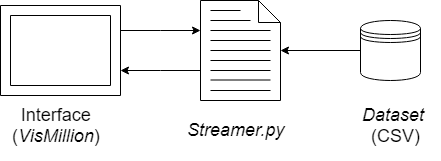
\includegraphics[width=0.9\linewidth]{Figures/server_Structure.png}
    \caption{System architecture}
        \label{fig:server_struct}
\end{figure}

\subsection{Dataset}
\label{subsection:dataset}
Since the purpose of this work is to use a large amount of data to be visualized in real-time the dataset to choose must follow two criteria: \textbf{Large} and \textbf{Time-based}. The most common datasets for this are event-based. This data has a timestamp associated (time-based) and one or more attributes, the events can be represented as packages that are sent to the client and then represented. The search of this type of data is facilitated by the exponential growth of technology \cite{6567202}, online shopping, social networks and, others that are always creating this kind of information that can be analyzed and fit perfectly in this case.

It was used two fonts to retrieve this kind of datasets: \textbf{Kaggle} and \textbf{Google BigQuery}. Each one contains multiple time-based data sources with large amounts of data. Using Google BigQuery, it was obtained data related Bitcoin transactions that suit entirely for the system purpose, with this dataset we are able to analyze trends and when there were more transactions occurring or not, as some anomalies that are not in the regular patterns.

The final dataset in CSV format contains hundreds of thousands of rows where which one corresponds to transaction value with a timestamp associated. Note this dataset contains only information about half a day of the whole dataset which can be found in Google BigQuery.

\subsection{Usability Tests Server Update}
\label{subsection:usabilityTests}
Due to the need for usability tests to evaluate the system, the server implementation was changed to support data timestamps, so the server could send the data like in a real scenario with different delays between the data dispatch. The retrieved data from the CSV file has now one required field beside the package value, the delta milliseconds between the next package. The server uses this value to set the thread sleep interval between each message sent to the client. This implementation makes more sense than the first one because in the previous approach the interval between each message was always the same, this it's very unlikely to happen in a real-world context.

\subsection{Dataset Generator}
\label{subsection:datasetGenerator}
The dataset generator is a script created due to the need to replicate the exact same views in usability test phase. This script generates CSV files with a pair of value and \textit{delta}. The dataset is processed by the server and then the packages are sent with the interval specified by the value of \textit{delta}. The generator reads the functions called by the user with some parameters and will output a dataset. These functions are:
\begin{itemize}
    \item \textbf{Linear\_Generation} - Generate data points following a linear regression between a given time interval and with a value range (from - to).
    \item \textbf{Constant\_Generation} - Generate data points given a time interval and with a value range.
    \item \textbf{Mark\_Outlier} - Append a outlier to the dataset.
\end{itemize}
For Linear\_Generation and Constant\_Generation the user must provide the size of that generation, this will create the number of packages given by this parameter.\newline 
The values generated by this functions are always randomly generated, using different inputs we can specify how sparse the data points can be and the chance of generate data outside the given value range (Alfa Random) and its limit (Prob Int).

\begin{figure}[h]
    \centering
    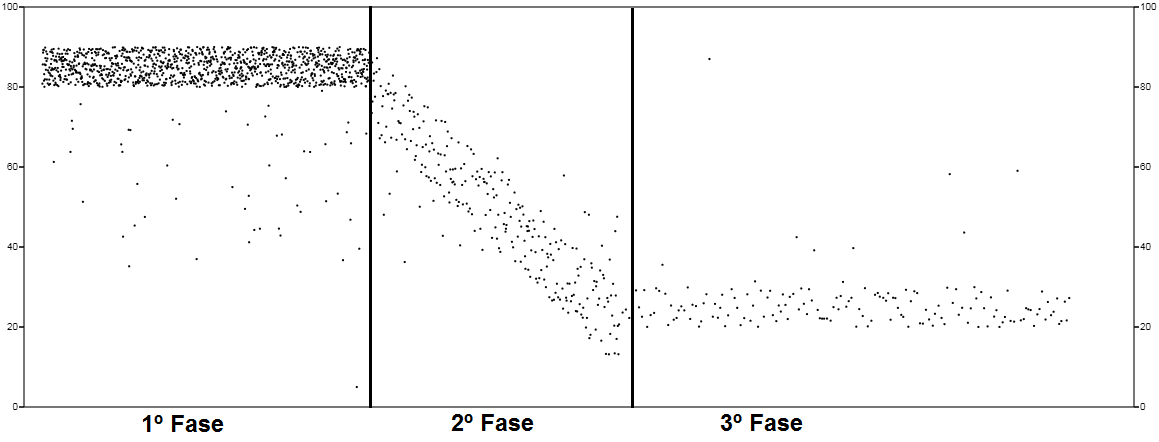
\includegraphics[width=\linewidth]{Figures/exemplo_datageneration.png}
    \caption{Generated \textit{dataset} - Example}
        \label{fig:example_datageneration}
\end{figure}

Figure \ref{fig:example_datageneration} demonstrates a generated dataset using Constant\_Generation on the first phase, followed by a Linear\_Generation and then a Constant\_Generation.

%\section{Background - InfoVis}
%\label{section:background}

\section{Front End - Visualization}
\label{section:frontend}
This application use D3 framework \cite{2011-d3} to help the creation of the dynamic visualizations. The system only supports one dimensional variables (without including its timestamp). 

The first thoughts about the interface began with the idea that the data should have a graceful degradation over time. Recent data should be way more detailed than old data because there are some characteristics that the users must be aware of during its analysis. As the information navigates through the interface packages are aggregated over some statistical methods such medians, averages, quartiles, frequencies, and others, so the user can be focused on the latest information without losing the context of information that has already been received.

Using this approach emerged a system based on visualization modules, each one presents the information in a different idiom allowing the client to have a more comprehensive experience of the information they are analyzing. The modules arranged side by side aim to create an innovative experiment in the investigation of datasets.

The connection between modules allows that information flows through them from right to left. The side by side approach creates a continuous vision about the system and connects all the information received, helping the analysis of the user in all data flow using different metrics in different moments of the chart. This method allows other users being able to develop other modules for they monitoring systems accordingly their sights and data domain.

It was implemented 3 modules: \textit{Linechart}, \textit{Barchart} and \textit{Scatterchart}. Each one represents one visualization idiom. The goal was to found navigation methods that allow the user to understand the data flow in real time, each one presents different metrics, scattercharts draw points that represent each package, linecharts represents the data tendencies and barcharts (or histograms) the information aggregation between values.
Each time the packages pass through a new module they are aggregated in some way and they should be transformed using smooth animations to their new form making that "graceful degradation" and letting the user won't be misled by abrupt disappearances or changes in the elements. 

For the interaction with each module, it was decided that the interface should be as simple as possible and not lead the user to a complex exploration of the information. The user is able to mouseHover the interface, this triggers a tooltip of the corresponding module and displays the information of the overlapping elements. Since this information is always moving (real-time), it was decided that this information should not be updated as the elements navigate through the chart, otherwise the user would have more difficulty tracking the mouse by the elements. This means that tooltip information is only updated when there is mouse movement created by the user.

In one hand, the visualization of the global chart allows an analysis that corresponds to free exploration of the information. On the other hand, the module visualization allows the user to make another search tasks depending on the type of data that the user wants to extract from a specific idiom. Searches can be done by time interval or directly orientated of the median values, using different methods there are some characteristics that can be found as anomalies or data aggregations. \newline 
These methods allow requirements like \textit{Expressiveness} and \textit{Effectiveness} \cite{Mackinlay} to be successfully followed since the main purpose of the system is that user won't be lost in its data visualization navigation and can have explicit information about the data visualized by modules.

\subsection{Implementation}
\label{subsection:implementation}
In the first implementation approach, it was used SVG elements to create the charts. Due to the lack of scalability (when it comes about large amounts of data) there was a need to rethink how the web interface should behave and how was going to be implemented in order to allow large amounts of data. The final solution was reached using \textit{canvas} API that allows users to draw elements in a rectangle using \textit{Javascript} to make the processing along with D3 framework. Despite this solution has better performance results than manipulating SVG elements, D3 does not support element animations on \textit{canvas}.


The class architecture for the system is presented at \ref{fig:uml}, the main class is called \textbf{Chart} and it is responsible to coordinate all the modules that belong to it and with the server, data is stored at this module and afterward filtered to each component. Since the interface follows the \textit{Update \& Draw} architecture there are 3 fundamental methods on these classes, \textbf{Chart} makes those calls for each module that exists. There is an abstract class called \textbf{Module} and all other three modules inherit from it (linechart, scatterchart, linechart). The first method is \textit{Update} and represents the processing phase of the data for each module. The second method is \textit{Draw}, at this stage, all the elements from that component are printed to \textit{canvas}. The last method is the \textit{mouseHover} event that triggers a tooltip and presents the information about the hovered element. 

\begin{figure}[h]
    \centering
    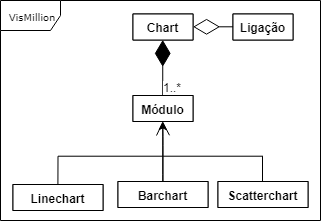
\includegraphics[width=0.8\linewidth]{Figures/uml.png}
    \caption{UML classes from \textit{VisMillion}}
        \label{fig:uml}
\end{figure}

The \textbf{Connection} component is an extension from Chart that creates the communication between the server and the interface, this class receives the packages and then appends it with a timestamp (if the packages do not come with one) to the data array saved by the \textbf{Chart}. This extension also allows the user to change the data flow in the testing phase.



\subsubsection{Chart}
\label{subsubsection:chart}

\begin{figure*}[ht]
    \centering
  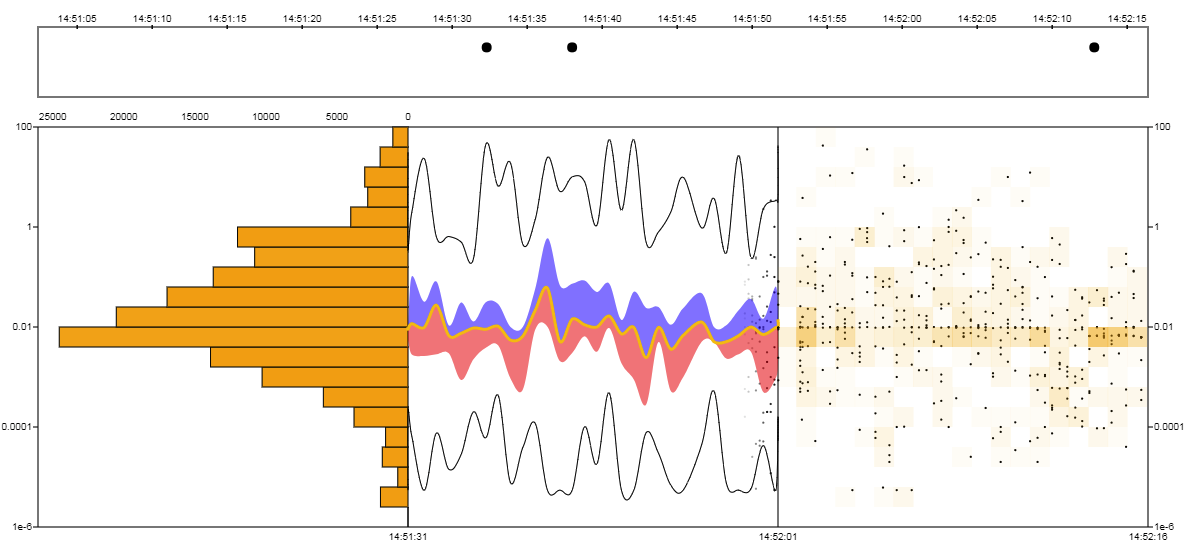
\includegraphics[width=\linewidth]{Figures/chart.png}
  \caption{Chart Overview}
  \label{fig:chart}
\end{figure*}

This system allows the interaction through all the modules so the \textit{Interactive Exploration} requirement can be ruled by this method. The data navigation implemented by the system let the locality of changes and preservation of the temporal context requisites being fulfilled by the interface.\newline
The chart is responsible to maintain these techniques align to each component, using the same scale function and domains to all the modules environments. These attributes are assigned by the users on the creation of the \textit{Chart} and usually cannot be updated in runtime. Figure \ref{fig:chart} represents a Chart and its modules.

\subsubsection{Modules}
\label{subsubsection:modules}
The initialization of each module have some global attributes that need to be set like \textit{deltaRange} that describes the time interval in seconds the module should present. The width is evenly distributed by all the modules of a Chart. In the update phase, each module asks the Chart for the data packages that are in its data interval. Since the packages navigate through each module from right to left the change between modules must be slowly degraded so the user won't lose its visualization context.

The implemented modules were carefully chosen given its visualization complexity (how familiar are the users to them and if the idiom is easy to understand). Globally, they complement each other well, and the required tasks can be executed with them: Flow and Trend analysis, identification of anomalies and non-typical aggregations, medians, max, min, etc.


\subsubsection{Barchart}
\label{subsubsection:barchart}
\textbf{Barchart} module does not need a time interval since its horizontal axis does not represent time like the other modules. Instead, it represents a frequency. For this reason, this module should be located the most left as possible. Each bar represents the number of packages received in a given data value interval, this will create a phenomenon of aggregation leads the user to understand the intervals where there are more packages with a certain value. \newline 
This approach takes into account the maintenance of the temporal context of all the information already received so far and making the information analysis more complete in a long term. Figure \ref{fig:barchart} shows a Barchart module.

As it is added new data to the bars, the bar that received a package blinks and grows slowly with a transition, so the user can understand the moments where new information is arriving at the module.

\begin{figure}[ht]
    \centering
    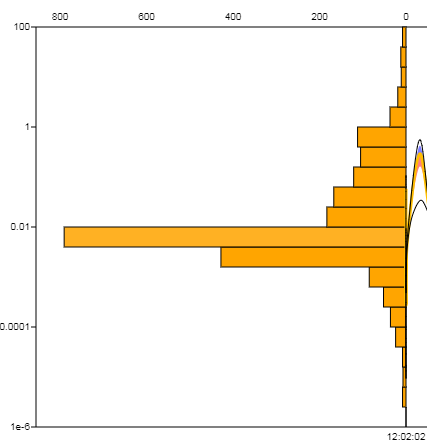
\includegraphics[width=0.8\linewidth]{Figures/barchart.png}
    \caption{Barchart}
        \label{fig:barchart}
\end{figure}

Using the \textit{mouseHover} function the user is able to get the interval of the values of the bar and the frequency of packages placed in that interval.

\subsubsection{Linechart}
\label{subsubsection:linechart}
With the \textbf{Linechart} module, the user is capable to understand patterns and tendencies about the information. The horizontal axis now represents the time interval set by the user. It was created a line connection between all the points that belong to the time interval. However, in high amounts of data, this approach wouldn't work because the user won't be capable to understand the condensed data points. So it were created two states, the \textit{high} and \textit{low} flow. Low flow connects all the packages, while High flow aggregates the data using \textit{Boxplots} approach, the module is divided by sections and then quartiles, median, max, and min are calculated for each section. After this calculations, a linechart connects all the sections with a different color for each metric creating a more understandable visualization. Figure \ref{fig:linechart} represents a linechart, where the top and bottom lines are the maximum and minimum values respectively. Median is given by the orange line and 1º quartile and 3º quartile by the red and purple colors.

\begin{figure}[ht]
    \centering
    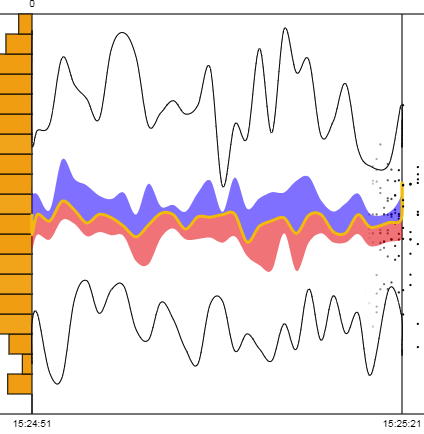
\includegraphics[width=0.8\linewidth]{Figures/linechart.png}
    \caption{Linechart}
        \label{fig:linechart}
\end{figure}

The interactions with this module shows the values for each attribute of a section.

\subsubsection{Scatterchart}
\label{subsubsection:scatterchart}
This visualization idiom can represent the data flow very easily, letting the user know what are the moments where exist more data incoming. This is the module that presents the most detailed information since all received packets are rendered. 

Like Linechart, Scatterchart also has the \textit{high} and \textit{low} flow states. The reason why this is needed is that there is a limit where FPS drop substantially, making the visualization not understandable anymore. The low flow state represents the all the packages received as a dot. The high flow state creates a heatmap in which the areas where the more colored the regions are the higher the concentrations of points will be. Unlike Linechart, the flow states in this module can coexist, overlapping each other and creating a simpler analysis of patterns.


\begin{figure}[ht]
    \centering
    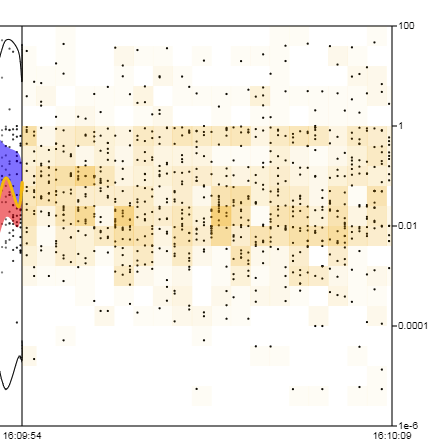
\includegraphics[width=0.8\linewidth]{Figures/scatterchart.png}
    \caption{Scatterchart}
        \label{fig:scatterchart}
\end{figure}

The interaction performed with this module results in the overlap of the mouse in the squares indicating the time interval and values associated with that packet as well as the number of elements contained in it.

\subsubsection{Outliers}
\label{subsubsection:outliers}
This module was created to represent the points that the user considers to be outliers. As in other works \cite{4015444}, this type of data is treated in separate views for a better understanding and coherence of the system. For this work, we consider the outliers are all values that are above the vertical domain defined by the user.

Being a component that does not require so much attention of the user (since the presence of these values must be atypical), the complexity of representation must be smaller than the other modules. This graphic is positioned at the top of the interface since the values represented in it are always larger than the domain (context maintenance).
The module occupies the entire width of the Chart allowing a more lasting visualization of the atypical values occurred.

The dots are represented along the chart and they have an animation in which it increases and decreases its radius so that it can be more easily identified by the user as it catches his attention. In order for the client to receive more details regarding each point, he must hover the mouse and get the information of the timestamp and value.


\section{Evaluation}
\label{section:evaluation}

VisMillion presents visualizations of large amounts of data in real time so that users can see trends, flows, and patterns occurring in the information. The layout of the side-by-side modules allows aggregation of the information over time, giving a temporal context of the overall dataset while allowing a more detailed description of the most recent packages.

\subsection{Usability Tests}
\label{subsection:usability}
Performing usability tests allows users to receive feedback from problems encountered in the programs and then make improvements or prove requirements. For this reason, these tests were performed, allowing to respond effectively to the proposed premises and to find implementation problems. The tests performed on a set of 21 users consisted of viewing the datasets generated by the script described in \ref{subsection:datasetGenerator}, tasks were created in order to infer the context of the users in the visualizations presented.

In the first phase, users are submitted to a questionnaire recognizing their characteristics and visualization abilities, so it is possible to perceive the level of skill of participants and find users who are more susceptible to errors. Subsequently, a demonstration is performed to the users and then four tests are done, each with a different purpose. In the end, users are asked to complete a final satisfaction questionnaire related to the tests.

The tests performed include the three types of visualization modules created. Barchart, Linechart, and Scatterchart from left to right, configured with a vertical domain in the range [0, 100] on a linear scale. Linechart and Scatterchart have a delta interval of 30 seconds and 15 seconds respectively. This way, the user is able to evaluate the different visualizations and it is possible to analyze if each module is useful and what the need to have different levels of information representation, from more detailed data to the right to its aggregation through statistical methods (such as medians and frequencies). The idea is who is viewing to be able to understand the data that is being received in real time while having an overview of all the information received so far without losing the context of it. \newline 
The testing phase uses the sales domain of a supermarket chain, the user is asked to identify items on each test and collect the timestamp of their responses.

The four tests are: 
\begin{itemize}
    \item \textbf{Trend Test} - This test consists in verifying the variation of the average values of sales occurred, in this way the user is able to identify the patterns and changes in sales figures. The user should identify the times when a variation in the average sales value happen, that is, when there is an increase, decrease or continuous moment of the data.
    \item \textbf{Outlier Test} - This test represents the analysis of the outliers and atypical aggregations, the user must be able to identify the values of the outliers module and the atypical aggregates whose representation does not fit the natural pattern of the received mean values.
    \item \textbf{Flow Test} - In this test, the user is asked to identify the flow changes that exist during the reception of the information. For this, the user must analyze the dataset and in the moments in which it finds an increase or a decrease in the amount of data received per unit of time should indicate this change. The identification timestamp is also collected.
    \item \textbf{Open Test} - In this test, the user is asked to view a dataset and questions are asked throughout the test. Before starting this test, the user is asked to be aware of the variation of the flow and the average value of the sales. At the end of the visualization, these two parameters must be described. In the middle of the test, the user is asked to identify the sale with the minimum and maximum value received so far. Subsequently, the user is asked about the range of values where there were more sales.
\end{itemize}

Of the 21 users used, 85.7\% use computers every day, on average each user knows about 7 visualization idioms listed in the questionnaire.

In the first test half of the variations were detected by all users (1, 3 and 6), on the other hand, some users did not report some of the remaining variations. The moment of identification of each variation of users varies widely, we can verify this by the figure \ref{fig:boxplot1} and by the standard deviation, this variation can be due to the fact that the users use different modules for this analysis, Linechart allows to verify this variation by the median while the Scatterchart by Heatmap.

\begin{figure*}[ht]
    \centering
    \begin{minipage}[b]{0.32\textwidth}
        \centering
        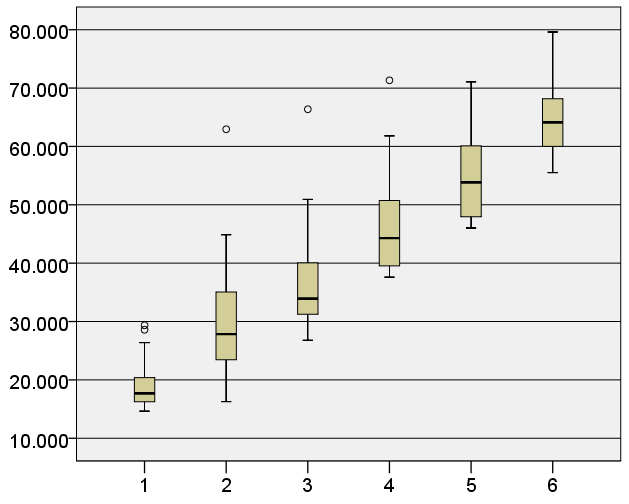
\includegraphics[width=\textwidth]{Figures/boxplot1_large.png}
        \caption{\textit{Boxplot} 1º test}
            \label{fig:boxplot1}
    \end{minipage}
    \hfill
    \begin{minipage}[b]{0.32\textwidth}
        \centering
        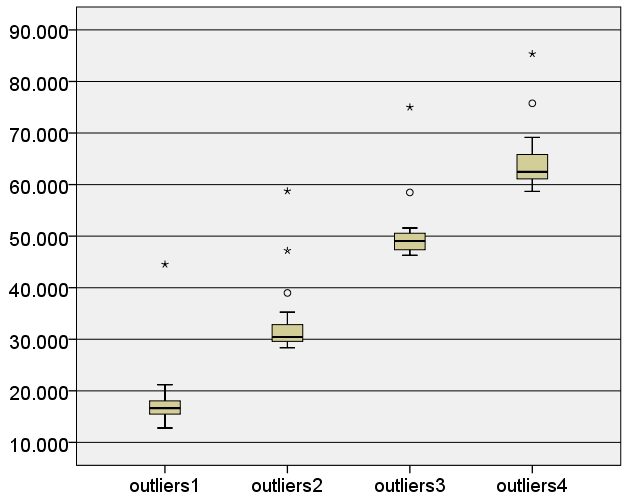
\includegraphics[width=\textwidth]{Figures/boxplot2_large.png}
        \caption{\textit{Boxplot} 2º test}
            \label{fig:boxplot2}
    \end{minipage}
    \hfill
    \begin{minipage}[b]{0.32\textwidth}
        \centering
        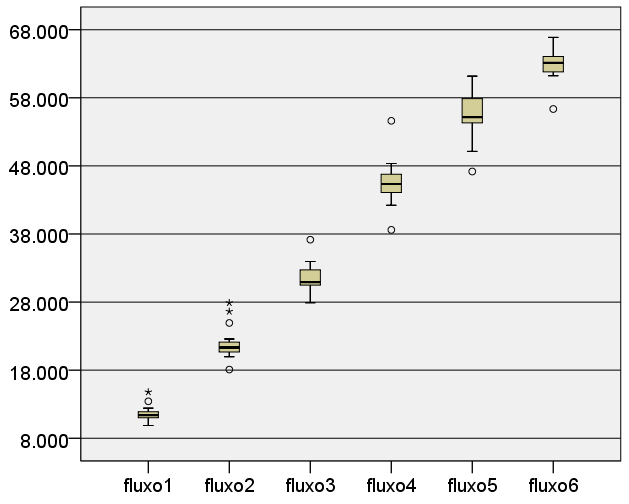
\includegraphics[width=\textwidth]{Figures/boxplot3_large.png}
        \caption{\textit{Boxplot} 3º test}
            \label{fig:boxplot3}
    \end{minipage}
    
\end{figure*}

The second task has a success rate above 95\% for all events. Since only one person failed to interpret outliers and atypical aggregations, this error may have been due to a lack of understanding of the task. In the figure \ref{fig:boxplot2} it is verified that for each event there were also between 1 and 2 outliers in the timely verification of the events. But most users had a uniform time between them. The confidence interval of all events varies between 5 and 7 seconds, with the standard deviation being relatively similar (between 6.279 and 7.273) which may mean that there is not much difference between the analysis of outliers and aggregations and that the instant they are found is a similar interval.

In the third test, the user success rate was always higher than 90\%, since the flow changes are easily analyzed by the Scatterchart heatmap, and checking the confidence interval of all events has no interval greater than 6 seconds. This means that average users identify changes in the rate of change of information quickly. From the figure \ref{fig:boxplot3} it is possible to see that there are also users who have identified these changes much earlier than the others.

In the fourth test, the question of identifying maximum and minimum values, 67\% of users correctly identified the minimum value and 76\% the maximum value.
The question regarding the range where there were higher sales, 90.5\% of users correctly answered that the range would be between 85 and 90. The two users who did not choose to respond in a correct way using a range spanning the correct range. \newline
Regarding the complete analysis of the dataset and the questions related to the flow and mean value, all users were able to correctly answer that the flow decreased over time while 95.2\% correctly answered the decrease in the variation of the mean value of the data. \newline
No user was wrong responding to the state of flow or variation, and only one forgot one of the states at the time of the question and could not remember again, derived from the remaining questions.


The final questionnaire regarding users satisfaction with the tests performed using closed-ended questions using rating scales from 1 to 5, the final questions allow the user to give suggestions and critics about the system and how the interface could be improved.
The close-ended questions were:
\begin{itemize}
    \item 1 - \textit{Are sales flow changes noticeable?}
    \item 2 - \textit{Is it easy to identify outliers in sales?}
    \item 3 - \textit{Is it easy to identify variations in average sales?}
    \item 4 - \textit{Is it easy to locate where there are larger sales aggregations?}
    \item 5 - \textit{Over time, it is perceptible the range of values in which there were more sales?}
    \item 6 - \textit{Is it easy to understand what which are the maximum and minimum sales values at a given time?}
    \item 7 - \textit{Is the transition from one module to another intuitive? }
    \item 8 - \textit{Is it easy to understand the time intervals of each module? } 
    \item 9 - \textit{Is the system easy to understand? }
    \item 10 - \textit{Is the system easy to interact with? }
    \item 11 - \textit{Is the system easy to learn? }
\end{itemize}

In questions 1 and 2 it can be seen that the majority of users answered 5 excepting some outliers (figure \ref{fig:boxplotQuest}), the standard deviation of 0.402 reveals the homogeneity of these responses.
The users considered that the visualization of the mean variations (question 3) is perceptible, its confidence interval varies between 4.39 and 4.85. In the questions related to checking flows and sales quantities (questions 4 and 5), users answered values between 4 and 5 and their standard deviation below 0.5 reveals a certain homogeneity in the sample. \newline
Question 6 about the verification of maximum and minimum points is the task with the lowest classification in relation to the others, and the median is 4, its standard deviation is also the highest (0.873), concluding that some of the users found the task less difficult than others. \newline
Users found that switching between languages is intuitive, giving a rating with a confidence interval between 4.4 and 4.93.
The last three questions have very similar values, with the means (5 for all) being relatively close and their confidence intervals also, concluding that the system is easy to interact, understandable and easy learn for users who are unfamiliar with the domain of application.
We can also check by the boxplots (fig. \ref{fig:boxplotQuest}) that from question 1 to 5 there were no ratings below 4 and that only question 6 contains a rating of 2. The remaining have minimum values at 3 and all of them have the third quartile at 5.

\begin{figure}[ht]
    \centering
    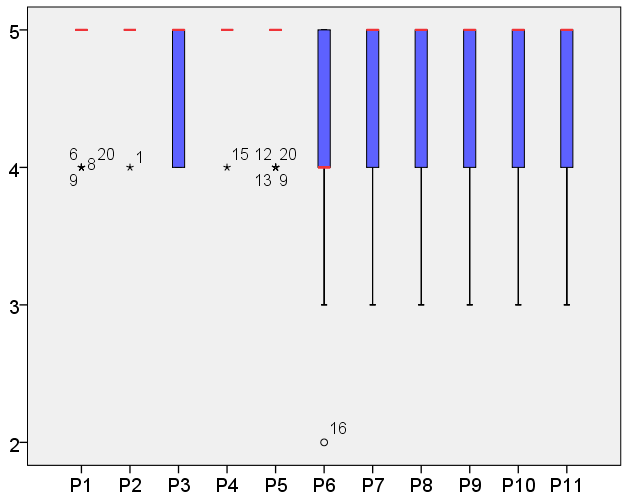
\includegraphics[width=\linewidth]{Figures/boxplot_quest.png}
    \caption{Close-ended questions results}
        \label{fig:boxplotQuest}
\end{figure}

To the opened question users were asked about: 
\begin{itemize}
    \item 1 - \textit{What were the biggest difficulties using the interface?} 
    \item 2 - \textit{What were the aspects that you find more intuitive in the interface?}
    \item 3 - \textit{What kind of improvement or suggestions do you have for the system?}
\end{itemize}

In the first question, users talked about the fact that the mouseHover interaction on the elements is difficult since the information was always moving, other user revealed some difficulty understanding the intersection between Linechart to Barchart as the bars grew automatically.

Regarding the second question, the greatest consensus that existed was the ease analysis of flow variations and mean values, as well as the identification of outliers. There were also users who showed that the use of different modules allowed comparing the information at different time intervals and that the analysis of large amounts of information is facilitated by the modules used. Another user reported that visualization of different languages allowed different statistical measures (averages, quartiles, maxima, minima) to be analyzed from the same sets of information and that this was a beneficial aspect of the interface.

About the third question, some users suggested that the interaction should be easier and the idea of creating a section with the data and moments that the user wanted to save for later analysis (like a bookmark of data).

In the end, a question was asked about if the system would fit into large-scale event monitoring. All users replied yes, this concludes that non-experienced users were able to understand a system for analyzing large amounts of information in real time.

\begin{figure*}[!ht]
    \centering
    \begin{minipage}[b]{0.48\textwidth}
        \centering
        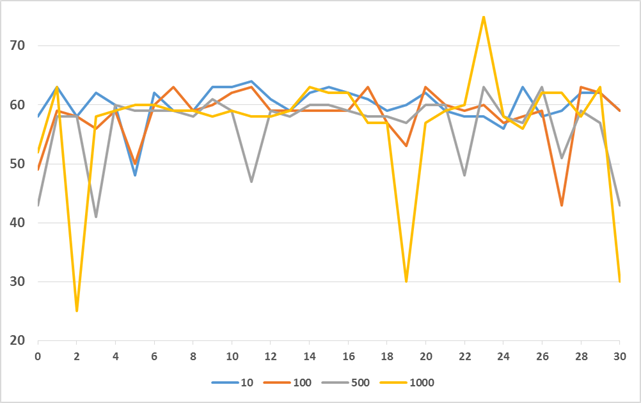
\includegraphics[width=\textwidth]{Figures/fps1.png}
        \caption{FPS - 1st Approach}
            \label{fig:fps1}
    \end{minipage}
    \hfill
    \begin{minipage}[b]{0.48\textwidth}
        \centering
        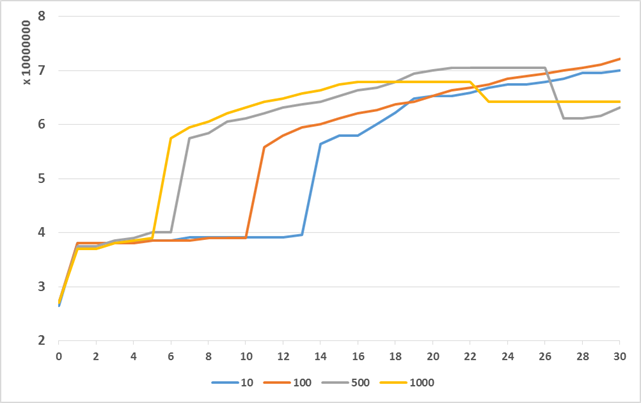
\includegraphics[width=\textwidth]{Figures/mem1.png}
        \caption{Memory Used - 1st Approach}
            \label{fig:mem1}
    \end{minipage}
\end{figure*}

\subsection{Performance Tests}
\label{subsection:performance}
Performance tests are important insofar as the high amount of information can slow the system to the point where there is not enough fluidity for an understandable view of the information, processing, and rendering of multiple elements can lead to a weakening and falling number of frames per second.

We used two approaches for this tests, using the same dataset:
\begin{itemize}
    \item 1st Approach - Using Barchart and Linechart
    \item 2nd Approach - Using Barchart, Linechart and Scatterchart
\end{itemize}

There were used four types of flows (packets per second) corresponding to 10, 100, 500 and 1000 packages per second. Each analysis took 30 seconds individually. The measures observed were FPS (frames per second) and memory used over time. The charts presented shows these measures over time, the line colors represents the packages per second and the vertical axis represents the frames per second for FPS and bytes for memory used.

For the first approach, the FPS followed a similar distribution across all flows (figure \ref{fig:fps1}), and their range did not pass typically below the 30s, except for the highest debt (1,000 packets per second) that included the two lowest peaks per second.
For memory used (figure \ref{fig:mem1}), it was verified that the higher the rate, the faster the memory consumed increases and progressively it remains constant.

In the second approach, Scatterchart used both states of high and low debt. It is possible to verify (using figure \ref{fig:fps2}) that the debts of 10 and 100 are relatively constant while the remaining debts create a sharp descent early on, thus making the view less fluid compared to the previous test we can see that the Scatterchart module has a direct influence in this case. In relation to the memory used it is noted that there is a growth much earlier than in the previous test and that the higher the debt the faster the increase is.

\begin{figure}[!ht]
    \centering
    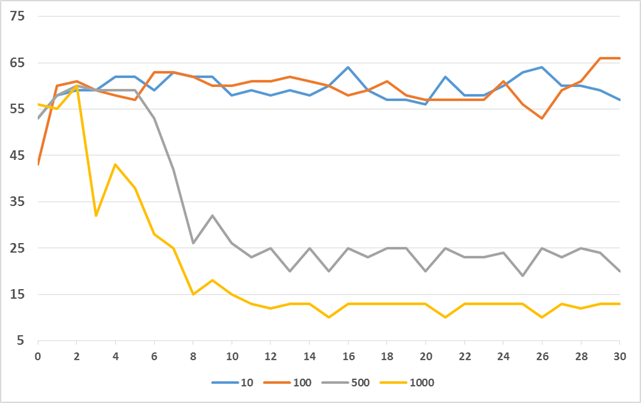
\includegraphics[width=\linewidth]{Figures/fps2.png}
    \caption{FPS - 2nd Approach}
        \label{fig:fps2}
\end{figure}

To test what is making the FPS drop substantially the low debt state was turned off, so the module only renders the heatmap corresponding to the density of values. The results at figure \ref{fig:fps3} show that plotting the points on the graph made the rendering of the module slow the whole system, since compared to the previous test, this test had a much higher result than the previous one, and the fluidity of the system was not compromised, because there was no fast descending of the FPS.

\begin{figure}[!ht]
    \centering
    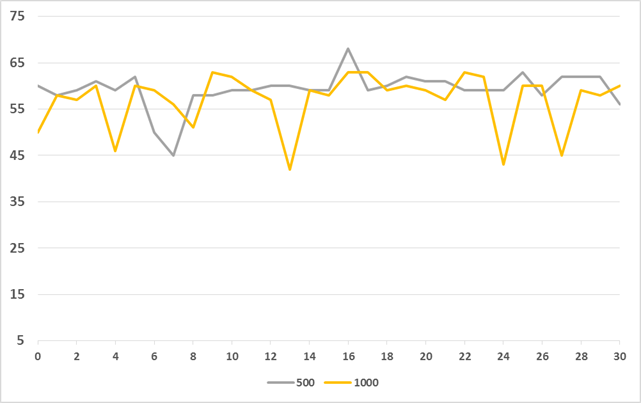
\includegraphics[width=\linewidth]{Figures/fps3.png}
    \caption{FPS - 2nd Approach (without low debit state)}
        \label{fig:fps3}
\end{figure}

\subsection{Discussion}
\label{subsection:discussion}
It was proposed a system that would perform an efficient representation of large amounts of data in real-time, taking into consideration that the application should be intuitive and that there was no loss of context by the user between the different phases of representation.

The users identified some things that can be improved like the interaction with the system, some mentioned that sometimes there were complicated tasks like following the elements with the mouse. On the other hand, most of them reported that the interface and the different modules allowed the analysis of different data at different times and that it was easy to analyze patterns and trends in information. Regarding the improvements, there were some ideas that could later be made in future work, always taking into account the proposed requirements.

In the end, all users agreed that this system would fit into a real case of monitoring large amounts of data in real time. Although it is only a prototype, the interface suggests that it is possible to perform this type of analysis through the solution found.

For the performance tests, the impact of the different modules was analyzed using the stated metrics (FPS and used memory). From there, it was concluded that the higher the flow rate, the greater the need for the modules to be adapted to efficiently respond to the amount of information received. In addition, the larger the number of modules available, the greater the memory used and consequently the interface performance can also decrease. By creating limits, it is possible to predict problems, without compromising user analysis.

% https://www.scribens.com/
% https://www.thesaurus.com/

\section{Conclusions \& Future Work}
\label{section:conclusions}
In this work study methods to visualize large amounts of data in real-time. It was verified that the greatest difficulties in this matter are the maintenance of the user's context to the changes, as well as the representation of a lot of information at the same time that leads to an overloading of the elements drawn by the interfaces of these systems. For this reason, there is a need to create approaches that address these difficulties by helping the user analyze patterns and occurrences in the transmitted data sets.

After the study of some systems and some paper drawings we created VisMillion, a visualization system for large amounts of data in real-time.  One of the major concerns of this work is to provide all this information representation without compromising the performance and efficiency of the system, the interface is able to adapt to the amount of information received and adapt to the existing flow at different moments of the visualization without there being jumps or abrupt interruptions that could lead the user to lose himself in his analysis of the data.

In order to test the system, we performed usability tests, including factors such as the analysis of patterns, trends, atypical values, aggregations, flow changes, etc. Feedback was obtained regarding the less positive aspects of the application, and most of them only showed some difficulty in interacting with the elements. On the other hand, most stated that the solution presented was simple and intuitive and that all the requested tasks were performed without much difficulty.

The system performance tests have been able to prove that the flow variation does not compromise the fluidity of the application and that despite the limitations of the web devices it is possible to perform an intuitive analysis without abrupt disruptions in data navigation. On the other hand, the implementation of the modules must always take into account the number of elements to render.

Based on the feedback we have received from the users we plan to improve our system making the interaction process easier and creating even more smooth transactions between the modules. Other feature that in the future would be interesting to implement with more detail a graceful degradation of information making the data transfer even more intuitive to the user.

Another aspect to introduce in this concept is the representation of multidimensional data, and for this aspect, a new study of the existing technologies involving the visualization of large amounts of multi-variable data would have to be carried out.

Systems such as VisMillion help users monitor their systems and find errors in real time so they can intervene as quickly as possible.

\addtolength{\textheight}{-12cm}   % This command serves to balance the column lengths
                                  % on the last page of the document manually. It shortens
                                  % the textheight of the last page by a suitable amount.
                                  % This command does not take effect until the next page
                                  % so it should come on the page before the last. Make
                                  % sure that you do not shorten the textheight too much.

%%%%%%%%%%%%%%%%%%%%%%%%%%%%%%%%%%%%%%%%%%%%%%%%%%%%%%%%%%%%%%%%%%%%%%%%%%%%%%%%



%%%%%%%%%%%%%%%%%%%%%%%%%%%%%%%%%%%%%%%%%%%%%%%%%%%%%%%%%%%%%%%%%%%%%%%%%%%%%%%%



%%%%%%%%%%%%%%%%%%%%%%%%%%%%%%%%%%%%%%%%%%%%%%%%%%%%%%%%%%%%%%%%%%%%%%%%%%%%%%%%




%%%%%%%%%%%%%%%%%%%%%%%%%%%%%%%%%%%%%%%%%%%%%%%%%%%%%%%%%%%%%%%%%%%%%%%%%%%%%%%%


\bibliographystyle{unsrt}
\bibliography{abstract.bib}

\end{document}
